\documentclass[14pt, twocolumn]{article}
\usepackage{hyperref}
\usepackage{amsmath}
\usepackage{amsthm}
\usepackage{tikz}
\usepackage[most]{tcolorbox}
\usepackage{geometry}
 \geometry{
 a4paper,
 total={170mm,300mm},
 left=25mm,
 right=25mm,
 top=26mm,
 bottom=26mm
 }

\usepackage{unicode-math}

% Set the main STIX Two fonts
\setmainfont{STIX Two Text}
\setmathfont{STIX Two Math}

% Tell LaTeX to use XITS Math whenever bold math is requested
\setmathfont{XITSMath-Bold.otf}[
  version=bold,
  Script=Math, 
  Style=TeX
]

\RequirePackage[scaled]{berasans}
\RequirePackage[semibold]{sourcecodepro}
\RequirePackage[scaled=.96,osf,sups]{XCharter}

\newtheorem{prop}{Prop.}
\newtheorem{ex}{Ex.}
\newtheorem{df}{Def.}
\newtheorem{thm}{Thm.}
\newtheorem{coro}{Corollary.}
\newtheorem{lemma}{Lemma.}

\newenvironment{tbox}{
    \begin{tcolorbox}[sharp corners, colback=white]
    
}{
    \end{tcolorbox}
}



\title{Realistic Galewsky Simulation}

\author{Haoyu Tang}


\begin{document}
\maketitle

\section{The Spectral Method}
\subsection{Preliminaries}
\subsubsection{Spherical Coordinate}

We use the following notation for the coordinate for $S^2$.
\begin{figure}[h]
    \centering
    

\tikzset{every picture/.style={line width=0.75pt}} %set default line width to 0.75pt        

\begin{tikzpicture}[x=0.4pt,y=0.4pt,yscale=-1,xscale=1]
%uncomment if require: \path (0,310); %set diagram left start at 0, and has height of 310

%Straight Lines [id:da9035231104008036] 
\draw    (224.67,202.83) -- (221.35,28) ;
\draw [shift={(221.32,26)}, rotate = 88.91] [color={rgb, 255:red, 0; green, 0; blue, 0 }  ][line width=0.75]    (10.93,-3.29) .. controls (6.95,-1.4) and (3.31,-0.3) .. (0,0) .. controls (3.31,0.3) and (6.95,1.4) .. (10.93,3.29)   ;
%Straight Lines [id:da98217303583292] 
\draw    (224.67,202.83) -- (86.98,274.08) ;
\draw [shift={(85.2,275)}, rotate = 332.64] [color={rgb, 255:red, 0; green, 0; blue, 0 }  ][line width=0.75]    (10.93,-3.29) .. controls (6.95,-1.4) and (3.31,-0.3) .. (0,0) .. controls (3.31,0.3) and (6.95,1.4) .. (10.93,3.29)   ;
%Straight Lines [id:da7834546523972832] 
\draw    (224.67,202.83) -- (383.51,258.1) ;
\draw [shift={(385.4,258.76)}, rotate = 199.19] [color={rgb, 255:red, 0; green, 0; blue, 0 }  ][line width=0.75]    (10.93,-3.29) .. controls (6.95,-1.4) and (3.31,-0.3) .. (0,0) .. controls (3.31,0.3) and (6.95,1.4) .. (10.93,3.29)   ;
%Straight Lines [id:da5891756328753197] 
\draw    (224.67,202.83) -- (264.2,83.74) ;
%Straight Lines [id:da7368878307157243] 
\draw  [dash pattern={on 0.84pt off 2.51pt}]  (264.2,83.74) -- (262.34,271.39) ;
%Straight Lines [id:da13183708755928825] 
\draw  [dash pattern={on 0.84pt off 2.51pt}]  (224.67,202.83) -- (262.34,271.39) ;
%Curve Lines [id:da3635789078184972] 
\draw    (195.4,217.99) .. controls (210.32,225.21) and (221.32,224.67) .. (232.5,221.07) ;
%Curve Lines [id:da5200419652502788] 
\draw    (232.88,175.76) .. controls (240.33,173.96) and (247.79,210.04) .. (232.5,219.07) ;

% Text Node
\draw (203.76,247.55) node [anchor=north west][inner sep=0.75pt]    {$\lambda $};
% Text Node
\draw (245.52,186.2) node [anchor=north west][inner sep=0.75pt]    {$\theta $};


\end{tikzpicture}

    \caption{Spherical Coordinate}
    \label{fig:sc}
\end{figure}

If we consider the differential, 
\begin{figure}[h]
    \centering
    

\tikzset{every picture/.style={line width=0.75pt}} %set default line width to 0.75pt        

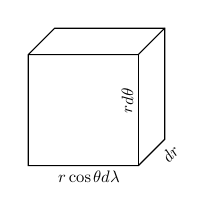
\begin{tikzpicture}[x=0.3pt,y=0.3pt,yscale=-1,xscale=1]
%uncomment if require: \path (0,300); %set diagram left start at 0, and has height of 300

%Shape: Cube [id:dp6183555325574622] 
\draw   (100,86.51) -- (131.71,54.8) -- (264.42,54.8) -- (264.42,188.56) -- (232.71,220.27) -- (100,220.27) -- cycle ; \draw   (264.42,54.8) -- (232.71,86.51) -- (100,86.51) ; \draw   (232.71,86.51) -- (232.71,220.27) ;

% Text Node
\draw (134.69,225.2) node [anchor=north west][inner sep=0.75pt]  [xscale=0.6,yscale=0.6]  {$r\cos \theta d\lambda $};
% Text Node
\draw (248.02,214.64) node [anchor=north west][inner sep=0.75pt]  [rotate=-311.53,xscale=0.6,yscale=0.6]  {$ \begin{array}{l}
dr\\
\end{array}$};
% Text Node
\draw (209.96,158.75) node [anchor=north west][inner sep=0.75pt]  [rotate=-271.45,xscale=0.6,yscale=0.6]  {$rd\theta $};


\end{tikzpicture}
    \caption{Spherical Differential}
    \label{fig:placeholder}
\end{figure}

then the differentials are:

\begin{table}[h]
    \centering
    \begin{tabular}{c|c|c|c}
            & $\lambda$  & $\theta$  & $a$ \\
            \hline \hline 
    Length  & $a\cos \theta$ & $a$ & 1 \\
    \hline 
    Area    & $a$ & $a\cos\theta $ & $a^2\cos\theta$ \\
    \end{tabular}
    \caption{Differential}
    \label{tab:scf}
\end{table}

To derive expressions for gradient, divergence and curl, we use the following boiler plate:
\begin{enumerate}
    \item (\textbf{Gradient}) Add $1/\text{length}$  before each term
    \item (\textbf{Divergence})  Add $1/\text{length}$; Modify the derivatives as $\frac{1}{\text{area factor}}\frac{\partial(\text{area factor})}{\partial q}$
    \item (\textbf{Curl}) Add $1/\text{length}$; Modify the derivatives as $\frac{1}{\text{length factor}}\frac{\partial(\text{length factor})}{\partial q}$

\end{enumerate}

The "area/length factor" is the part of the differential that involves the coordinate the derivative is taking with respect to. 
As a result, we have:
\begin{tbox}
    \begin{prop}
    The gradient of a vector field  $F$ is:
    $$
        \left(\frac{1}{a\cos \theta}\frac{\partial F}{\partial \lambda }, \frac{1}{a}\frac{\partial F}{\partial \theta} \right)^T
    $$
    The divergence of $\mathbf{v}$ is :
    \begin{equation}
    \nabla \cdot \mathbf{u} =\frac{1} {a\cos(\theta)} \frac{\partial u}{\partial \lambda}  + \frac{1}{a}\frac{1}{\cos\theta}\frac{\partial (v\cos\theta)}{\partial \theta}
    \end{equation}
    The z-component of curl of $\mathbf{v}$ is:
    \begin{equation}
        \zeta =  \frac{1}{a\cos \theta}\frac{\partial v}{\partial \lambda } -\frac{1}{a}\frac{1}{\cos \theta}\frac{\partial (\cos \theta u)}{\partial \theta} 
    \end{equation} 
\end{prop}

\end{tbox}
By taking the gradient and then the divergence, we get the laplacian:
\begin{tbox}
    \begin{coro}
        \begin{align*}
            L^2=
                          &= \frac{1}{a^2\cos^2 \theta}\frac{\partial^2}{\partial \lambda^2}  \\
                          &+ \frac{1}{a^2\cos\theta}\frac{\partial }{\partial \theta}\left(\cos  \theta  \frac{\partial}{\partial \theta}\right)
        \end{align*} 
    \end{coro} 
\end{tbox}




\subsection{Vorticity Equation for 2D Flow}
The vorticity equation  for incompressible, barotropic fluid is 

\begin{equation}
    \frac{D\boldsymbol{\omega}}{Dt}=(\boldsymbol{\omega}\cdot \nabla)\boldsymbol{v}
\end{equation}

In component form:
\begin{align*}
    \frac{D\omega^{(x)}}{Dt} &= \omega^{(x)}\partial_x u +
    \omega^{(y)}\partial_y u +
    \omega^{(z)}\partial_z u \\
    \frac{D\omega^{(y)}}{Dt} &= 
    \omega^{(x)}\partial_x v+
    \omega^{(y)}\partial_y v+
    \omega^{(z)}\partial_z v \\
    \frac{D\omega^{(z)}}{Dt} &= 
    \omega^{(x)}\partial_x w +
    \omega^{(y)}\partial_y w +\omega^{(z)}\partial_z w 
\end{align*}
For two dimensional flow, $\omega=(0,0,\zeta)$, and $\mathbf{u}=(u,v,0)$, hence the only surviving equation is the third equation:
\begin{equation}
    \frac{D\omega^{(z)}}{Dt}=\frac{D\zeta}{Dt}=0
    \label{eq:bve}
\end{equation} 
\subsection{The Stream Function}
Next we show that the field $\zeta$ contains all the information required to recover $\mathbf{v}$.

Since we assumed incompressibility, we have divergence-free velocity : $\nabla \mathbf{u}=0$, hence there exists a vector field $\mathbf{A}$ such that $\nabla \times \mathbf{A} =\mathbf{v}$. In particular, one can show that  we can choose $A^{(x)}=A^{(b)}=0$ so that $\partial_x A^{(z)}-\partial_y A^{(z)}=\omega^{(z)}=\zeta$. 

\begin{tbox}
    \begin{df}
        Define the \textit{stream function}  $\psi:\mathbb{R}^2\to\mathbb{R}$ as $-A^{(z)}$ where $\nabla \times \mathbf{A}=\mathbf{v}$. As a result, 
        $$
        \begin{cases}
            u= - \partial_y \psi \\
            v=\partial_x \psi
        \end{cases}
        $$
        Equivalently, it is the solution to the Poisson equation:
        \begin{equation}
            \nabla ^2 \psi = \zeta 
        \end{equation}
    \end{df}
\end{tbox}

Hence, instead of simulating a equation about $\mathbf{v}=(u,v)$, we simulate an equation about $(\zeta,\psi)$. The next subsection derives this equation from equation (\ref{eq:bve})

\subsection{Spherical Form}
\begin{itemize}
    \item We need rewrite 
    $
        \frac{D\zeta}{Dt}=0
    $
    in spherical form and replace terms involving $\mathbf{v}$ with the stream function $\psi$.
\end{itemize}

We attempt to represent the solution in a complete basis for $S^2\to \mathbb{R}$ known as the \textbf{spherical harmonics}

\subsection{Spherical Harmonics}
Consider the laplace equation in spherical coordinate:
$$
\nabla^2 \psi = 0 
$$
If we assume solution of the form $\psi(a,\lambda,\theta)=R(a)Y(\lambda,\theta)$, we can separate 
the variable. If we assume the separation constant is $\mu$ then the radial equation becomes:
\begin{equation}
    \left\{\color{purple}{\frac{1}{a^2\cos^2 \theta} \frac{\partial^2}{\partial \lambda^2}}  +
                          \color{brown}{\frac{1}{a^2\cos\theta}\frac{\partial }{\partial \theta}\left(\cos  \theta  \frac{\partial}{\partial \theta}\right)}  \right\} \psi = \mu\psi
\end{equation}
We note that this is an eigenvalue problem of the strucutre $L^2\psi = \mu \psi$. One can show that the spherical harmonics are
the solution to the eigenvalue problem:
\begin{tbox}
    \begin{df}
       Define spherical harmonics as:
        \begin{equation}
            Y_{n,m}(\lambda,\theta)=A_{n,m}P_{n,m}(\sin(\theta))\exp(im\lambda)
        \end{equation}
        where $A_{n,m} = (-1)^n\sqrt{\frac{2n+1}{4\pi}\frac{(n-m)!}{(n+m)!}}$ is the normalization factor 
        for orthonormilization.$P_{n,m}$ is the associated legendre pollnomials.
    \end{df}
\end{tbox}

\section{Appendix A. Background in Series-Approximation Method}
Consider a PDE:
\begin{equation}
    u_t = F(u)
\end{equation}
where $F$ is an operator involving spatial derivatives of $u$. 
The series-approximation method refers to (1) assume a series-expansion for the solution $u$ exists (2) Transform 
the PDE $u_t=F(u)$ to constraints on the coefficeints (3) Solve the resulting system to get the coefficients.
Concretely, we let:
$$
u(t,x)=\sum_{k=1}^N a_k(t) \phi_k(x)
$$
where $\{\phi_k\}$ are pre-determined basis functions that satisfy the boundary condition on the domain $\Omega$

\subsection{Exact Solution is Often Impossible}

\begin{ex}
    Consider the 1d equation with fourier basis $\{\exp{ikx}\}_{k=_N}^N$:
    \begin{equation}
        \frac{Du}{Dt} = 0
            \label{eq:DuDt}
    \end{equation}
    or, 
    $$\frac{\partial u}{\partial t}= -u\frac{\partial u}{\partial x}$$
    Now, substituting $u=a_k(t)\exp(ikx)$ into (\ref{eq:DuDt}), we get:
    \begin{align*}
        \frac{da_k(t)}{dt}(t)e^{ikx} &= -(a_ke^{ikx})(ika_ke^{ikx}) \\
    \end{align*}
    This gets us an over-determined system of ODEs:
    \begin{equation}
        \begin{align}`'
            \frac{da_k(t)}{dt} &=  -\sum_{k_1+k_2=k} ia_{k_1}a_{k_2} & k=-N...N \\
            0 &= \sum_{k_1+k_2>k}  ia_{k_1}a_{k_2} &
        \end{align}
    \end{equation}
    which is a total of $4N+1$ equations for $2N+1$ unknown functions. 

\end{ex}

\subsection{Galerkin Projection}
Instead, solvable system can be obtained if we only require the residual to be orthogonal to  
the basis, i.e.,
$$
\left\langle R,\phi_j \right\rangle = \left\langle \left\{\sum_{k=1}^N \frac{da_k}{dt}\phi_k - F\left(\sum_{k=1}^N a_k\phi_k\right)\right\},\phi_j \right\rangle =0
$$
Equivalently:
\begin{align*}
    \int_{\Omega} dx \left\{\sum_{k=1}^N\frac{da_k(t)}{dt}\phi_k(x) - F\left(\sum_k a_k(t)\phi_k(x)\right) \right\} \phi_j(x) &=0 \\
    \sum_{k} \left[ \int_{\Omega}\phi_j(x)\phi_k(x)dx\right] \frac{da_k(t)}{dt} = \int_{\Omega}  F\left(\sum_k a_k(t)\phi_k(x)\right)dx
\end{align*}
We can denote $M_{jk}=\int_{\Omega}\phi_j \phi_k dx$, then:
\begin{tbox}
    The Galerkin Projection creates a system of $N$ ODES of $N$ equations, $\forall j=1...N$, we have:
    \begin{equation}
        \sum_k M_{jk} \frac{da_k(t)}{dt} = \int_{\Omega}  F\left(\sum_k a_k(t)\phi_k(x)\right)dx 
        \label{eq:gp}
    \end{equation}
\end{tbox}

\subsection{Spectral Method}
The spectral method requires the basis to be orthogonal. Therefore \ref{eq:gp} reduces to:
\begin{equation}
    \frac{da_j(t)}{dt} = \frac{1}{M_{jj}}\int_{\Omega}  F\left(\sum_k a_k(t)\phi_k(x)\right)dx 
\end{equation}





\end{document}